\PassOptionsToPackage{numbers,square,sort&compress}{natbib}
\documentclass[11pt,twocolumn]{article}

\IfFileExists{acl.sty}{
  \usepackage[review]{acl}
}{
  \usepackage[margin=0.72in,columnsep=0.24in]{geometry}
  \usepackage[numbers,square,sort&compress]{natbib}
}

\usepackage{times}
\usepackage{latexsym}
\usepackage[T1]{fontenc}
\usepackage[utf8]{inputenc}
\usepackage{microtype}
\usepackage{inconsolata}
\usepackage{graphicx}
\usepackage{booktabs}
\usepackage{amsmath}
\usepackage{float}
\usepackage{placeins}
\IfFileExists{xurl.sty}{\usepackage{xurl}}{\usepackage{url}}
\setcitestyle{numbers,square}
\makeatletter
\@ifpackageloaded{hyperref}{}{\usepackage[hidelinks]{hyperref}}
\makeatother

\graphicspath{{figures/}}

\title{Predicting Ideology from Social Media Content Using Weakly Supervised Transformer Models}

\author{Jacob Kim and Billy Fox \\
  Rochester Institute of Technology \\
  \texttt{jck9187@rit.edu, bcf7023@rit.edu}}
\date{}

\begin{document}
\maketitle

\begin{abstract}
This project studies whether social media text can support political ideology prediction beyond a single left-right label. The system predicts whether a post is politically relevant, what issue target it discusses, what stance and frame it uses, and whether its ideology is economically left or right, socially liberal or conservative, intense, or ambiguous. The completed real-data experiment uses MITweet with a balanced TF-IDF baseline and a pretrained RoBERTa baseline. Both beat random performance, but RoBERTa does not uniformly outperform TF-IDF: it improves social-direction prediction while overpredicting the majority neutral class for economic direction. The B5 and B6 experiments currently verify the flat and hierarchical model pipeline on a small smoke run rather than proving final model quality. The main result is that label balance, data access, and careful evaluation matter before stronger claims can be made about transformer architecture.
\end{abstract}

\section{Introduction}

Ideology detection is the task of predicting political viewpoints from text. This is useful because political discussion now happens at large scale on social media, where researchers may want to study public opinion, ideological polarization, and how communities react to policy debates. A simple classifier might ask whether a post is liberal or conservative. This project studies a harder version of that task. A post can be relevant or irrelevant to politics, aimed at a particular policy target, supportive or opposed to that target, framed around economic or social concerns, and still be mixed or ambiguous. In this paper, ``harder'' means that the model must predict several connected labels rather than only one overall ideology class.

The main research question is whether weakly supervised transformer models can predict multidimensional ideology from social media text while remaining useful when topics, communities, or platforms change. This question comes directly from MITweet, which argues that ideology should be modeled through multiple facets instead of collapsed into a single axis \cite{liu-etal-2023-ideology}. It is also motivated by work showing that ideology classifiers can learn topic shortcuts when supervision is scarce or biased \cite{chen-etal-2023-ideology}. For example, a model may learn that certain words are common in one party's posts instead of learning how a stance is being expressed.

The planned system combines high-quality labels with larger weakly labeled data. MITweet provides carefully annotated labels for ideological relevance and ideological direction across facets. Reddit Political Compass provides weaker signals along economic and social axes. Reddit Politosphere provides broad political subreddit text and community structure, but it does not directly provide post-level ideology labels in the same form as MITweet. In our design, Politosphere is used as a source of political text and community shift, while weak labels are derived from community metadata, lexicons, and Political Compass supervision rather than treated as gold ideology labels.

The strongest completed empirical result comes from MITweet because Politosphere access was blocked in the available environment. The Reddit branch is therefore implemented and smoke-tested, but not fully evaluated at the intended scale. On MITweet, a pretrained RoBERTa model helps when labels are reasonably balanced, as they are for social direction. It struggles when one class dominates, as it does for economic direction. The smaller smoke run also shows that the hierarchical B6 model is not automatically better than the flatter B5 model under limited training. These results make the next step clear: use class-weighted or focal loss for the ideology heads and rerun the full weak-supervision experiment when the Reddit data is reachable.

\section{Related Work}

This project depends most directly on MITweet, Reddit Politosphere, Reddit Political Compass, and work on biased supervision. MITweet is the main gold-label source because it annotates ideology as a set of facets rather than a single party or left-right label \cite{liu-etal-2023-ideology}. That design shapes our prediction heads for relevance, economic direction, and social direction. It also gives a concrete way to test whether a model can learn ideological direction from short social media posts.

Reddit Politosphere is useful for a different reason. It is a large text and network resource covering political subreddit discussion over time \cite{hofmann-etal-2022-politosphere}. We do not treat Politosphere as if it already contains the same post-level ideology labels as MITweet. Instead, it supports the planned weak-supervision and robustness setting: train on broad Reddit political language, then test whether the model generalizes across communities. Reddit Political Compass is closer to our label space because it studies economic and social ideology axes on Reddit \cite{colacrai-etal-2024-politicalcompass}. That makes it a natural weak-supervision source for the economic-direction and social-direction heads.

Prior modeling work explains why these datasets should not be used only with random train-test splits. Chen et al. show that ideology prediction can overfit the topic of a post rather than the way ideology is expressed \cite{chen-etal-2023-ideology}. This directly motivates our planned leave-topic-out, leave-community-out, and cross-platform checks. RoBERTa is used as the transformer encoder because it is a strong general text representation model \cite{liu2019roberta}, but the results here show that a transformer still needs loss functions and sampling strategies that match the label distribution. Simpler lexical and sequence baselines also remain important because older political text classification work shows that non-transformer models can be competitive when lexical cues are strong \cite{chang-masterson-2020-wordorder}.

Disagreement-aware learning is also relevant. Work on learning with disagreements treats annotator variation as signal rather than noise \cite{leonardelli-etal-2025-lewidi}. That matters for political text because a post can be genuinely mixed, sarcastic, or unclear. In our setting, a hard label is the single majority class used for ordinary classification. A soft label is the full annotator distribution over classes. Soft labels let the model learn that a post split between support and mixed is different from a post where every annotator agreed.

\section{Methodology}

The project models ideology through eight prediction heads: relevance, target, stance, frame, economic direction, social direction, intensity, and ambiguity. Relevance identifies whether a post is political. Target identifies the issue or actor discussed by the post. Stance indicates support, opposition, or a mixed position toward the target. Frame captures the type of reasoning used, such as economic, social, security, rights, or other framing. Economic direction and social direction map the post onto two ideology axes. Intensity captures how strong the ideological signal is, and ambiguity captures whether the label is uncertain or mixed.

For the real-data experiment, MITweet labels were projected into the heads that the dataset can support cleanly. The local MITweet file contains 12,594 labeled posts. Relevance is positive when any MITweet ideology facet is marked relevant. Economic direction is derived from MITweet's economic facets, and social direction is derived from its social facets. If no facet on an axis is active, the projected label is neutral. This projection lets MITweet evaluate relevance, economic direction, and social direction, but it does not fully evaluate target, stance, frame, intensity, or ambiguity.

For the Reddit branch, the codebase implements ingestion, weak-label construction, annotation folding, counterfactual editing, model training, prediction export, calibration, paired bootstrap testing, and error analysis. The intended weak-supervision stage uses larger Reddit resources to teach the model political language patterns before gold fine-tuning. This is the part of the project that operationalizes combining datasets: MITweet supplies clean labels, Reddit Political Compass supplies weak economic and social signals, and Politosphere supplies broader political communities for robustness tests.

B1 is a TF-IDF logistic-regression baseline with balanced class weights. B2 is a RoBERTa-base classifier fine-tuned on the available MITweet labels with ordinary cross-entropy. B3 through B5 are flat transformer variants intended for weak pretraining and gold fine-tuning. B5 adds decomposition heads for target, stance, frame, intensity, and ambiguity. B6 is the hierarchical representation model. It maps text into a latent ideology representation and jointly predicts discourse and ideology heads. The purpose of B6 is to test whether modeling discourse structure helps ideology prediction, not just whether a larger model improves the score.

\section{Experimental Design}

The original experimental design evaluates whether the final model generalizes across topics, communities, and platforms. The completed real-data experiment compares B1 and B2 on MITweet with three random seeds. Evaluation uses macro-F1 because the ideology labels are imbalanced. The comparison also uses paired bootstrap testing over shared validation posts, which estimates whether one model outperforms another after resampling examples with replacement. Calibration is evaluated by comparing model confidence on correct and incorrect predictions.

Table~\ref{tab:mitweet} shows the real MITweet results. Both B1 and B2 beat random performance. B2 does slightly better on relevance and social direction, but B1 does better on economic direction. The economic-direction split explains why. About 91\% of the economic labels are neutral. Across seeds, B2 reaches high F1 for the neutral class but near-zero F1 for the left and right classes. B1 handles those minority classes better because it uses balanced class weights.

\begin{table}[t]
\centering
\small
\begin{tabular}{lccc}
\toprule
Label & B1 TF-IDF & B2 RoBERTa & Random \\
\midrule
Relevance & $0.708 \pm 0.077$ & $0.743 \pm 0.064$ & $\sim 0.41$ \\
Economic & $0.459 \pm 0.021$ & $0.341 \pm 0.017$ & $\sim 0.21$ \\
Social & $0.534 \pm 0.015$ & $0.579 \pm 0.022$ & $\sim 0.34$ \\
\midrule
Mean & $0.567 \pm 0.033$ & $0.554 \pm 0.024$ & $0.314$ \\
\bottomrule
\end{tabular}
\caption{Three-seed MITweet results. Values are macro-F1 mean and standard deviation.}
\label{tab:mitweet}
\end{table}

\begin{figure}[t]
    \centering
    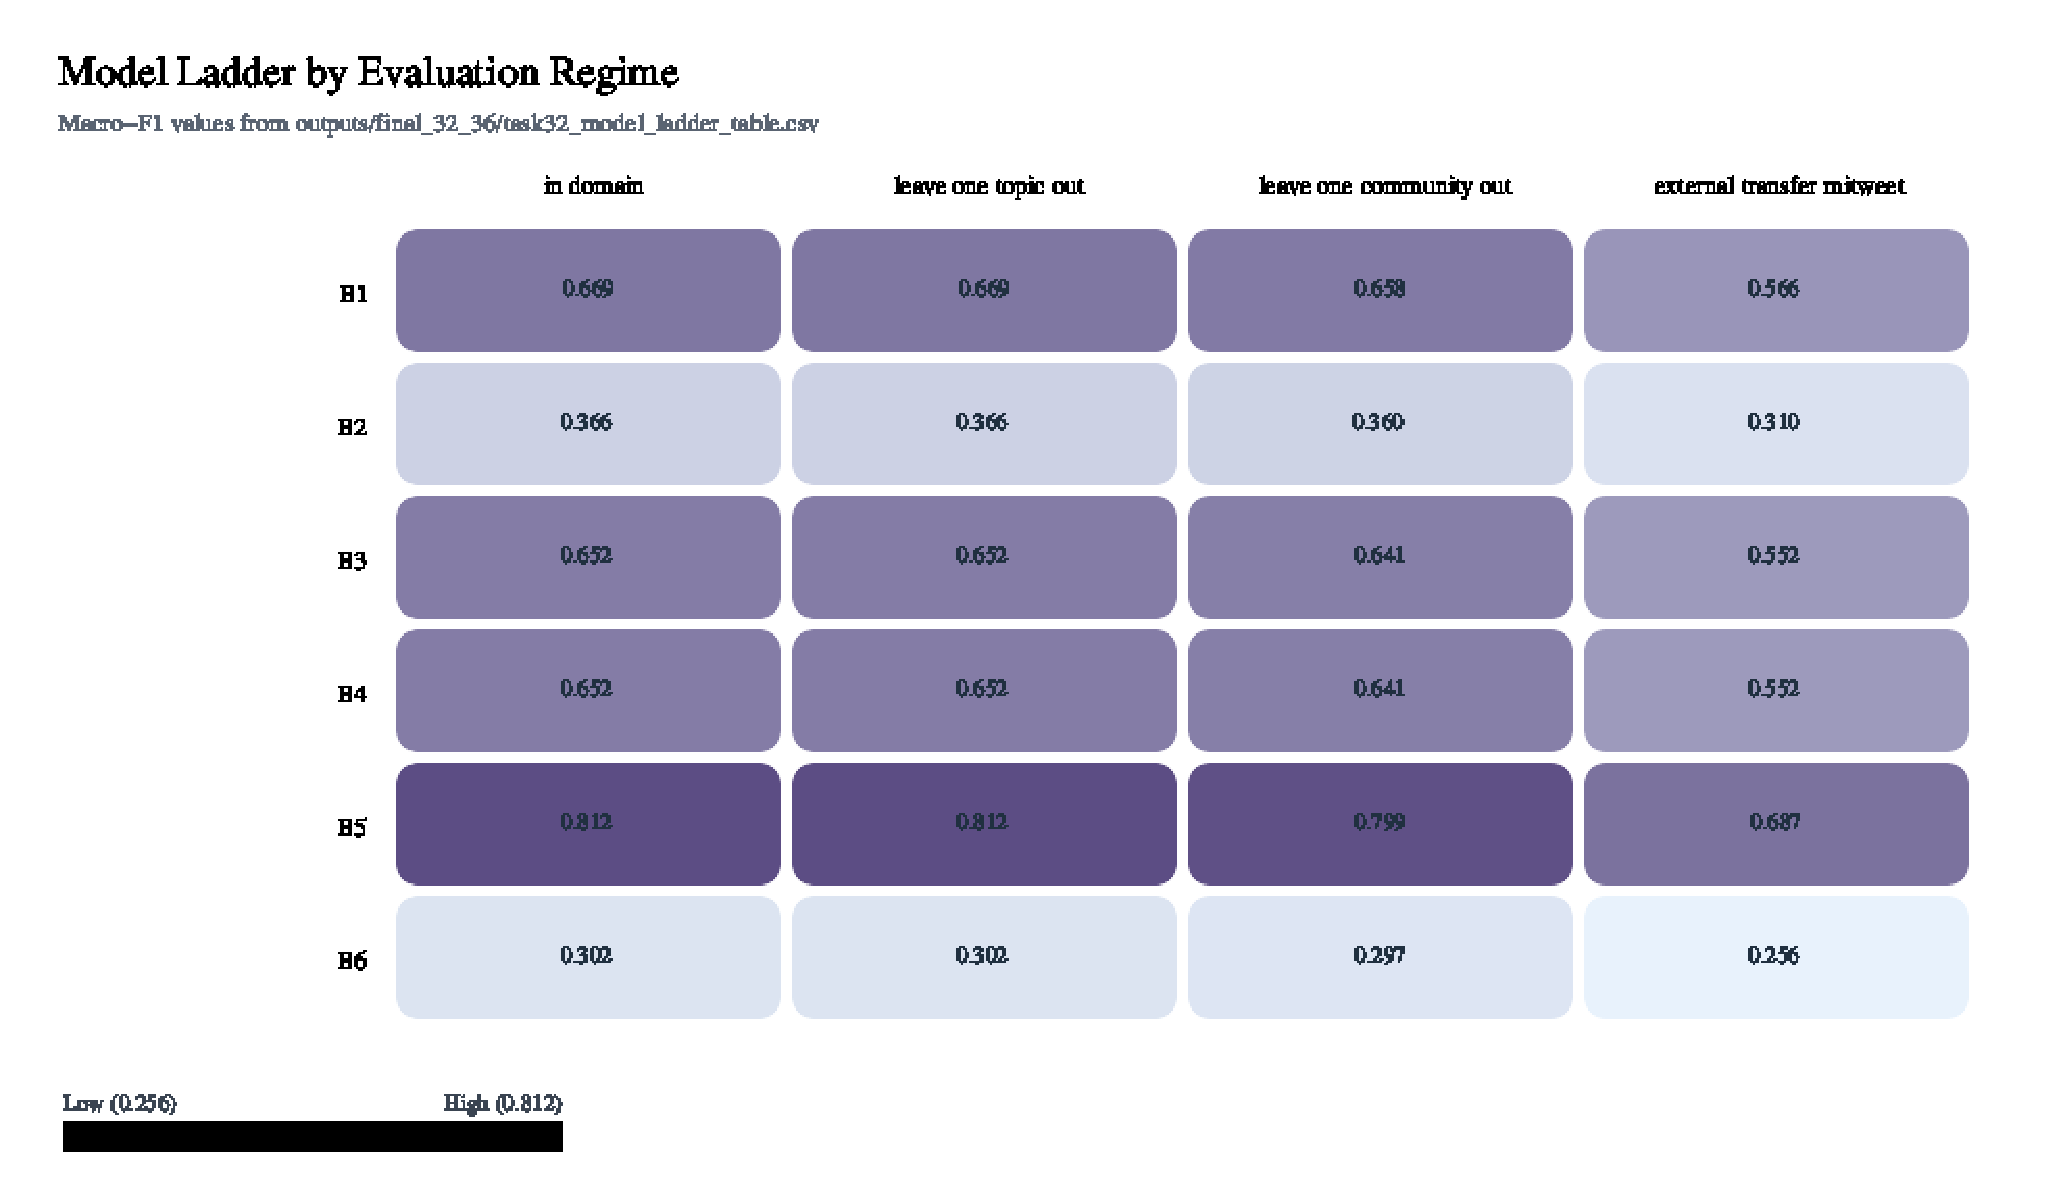
\includegraphics[width=\columnwidth]{figure01_model_ladder_heatmap.pdf}
    \caption{Macro-F1 by model and evaluation regime.}
    \label{fig:ladder}
\end{figure}

The paired bootstrap comparison gives the same interpretation. B1 significantly beats B2 on economic direction for all three seeds. On social direction, B2 beats B1 for one seed and ties for the other two. This means RoBERTa is useful when the label distribution gives it enough signal, but it is not robust to imbalance by default.

\begin{table}[t]
\centering
\small
\begin{tabular}{lccc}
\toprule
Label & Correct & Error & Gap \\
\midrule
Relevance & 0.957 & 0.849 & +0.107 \\
Economic & 0.959 & 0.791 & +0.168 \\
Social & 0.686 & 0.577 & +0.109 \\
\bottomrule
\end{tabular}
\caption{B2 confidence on correct and incorrect MITweet predictions.}
\label{tab:confidence}
\end{table}

Table~\ref{tab:confidence} shows that correct B2 predictions are more confident than errors for every projected MITweet label. This is useful because an abstaining classifier only helps when confidence is meaningfully different on correct and incorrect cases. The largest gap appears for economic direction, which is also the weakest RoBERTa result.

\begin{figure}[t]
    \centering
    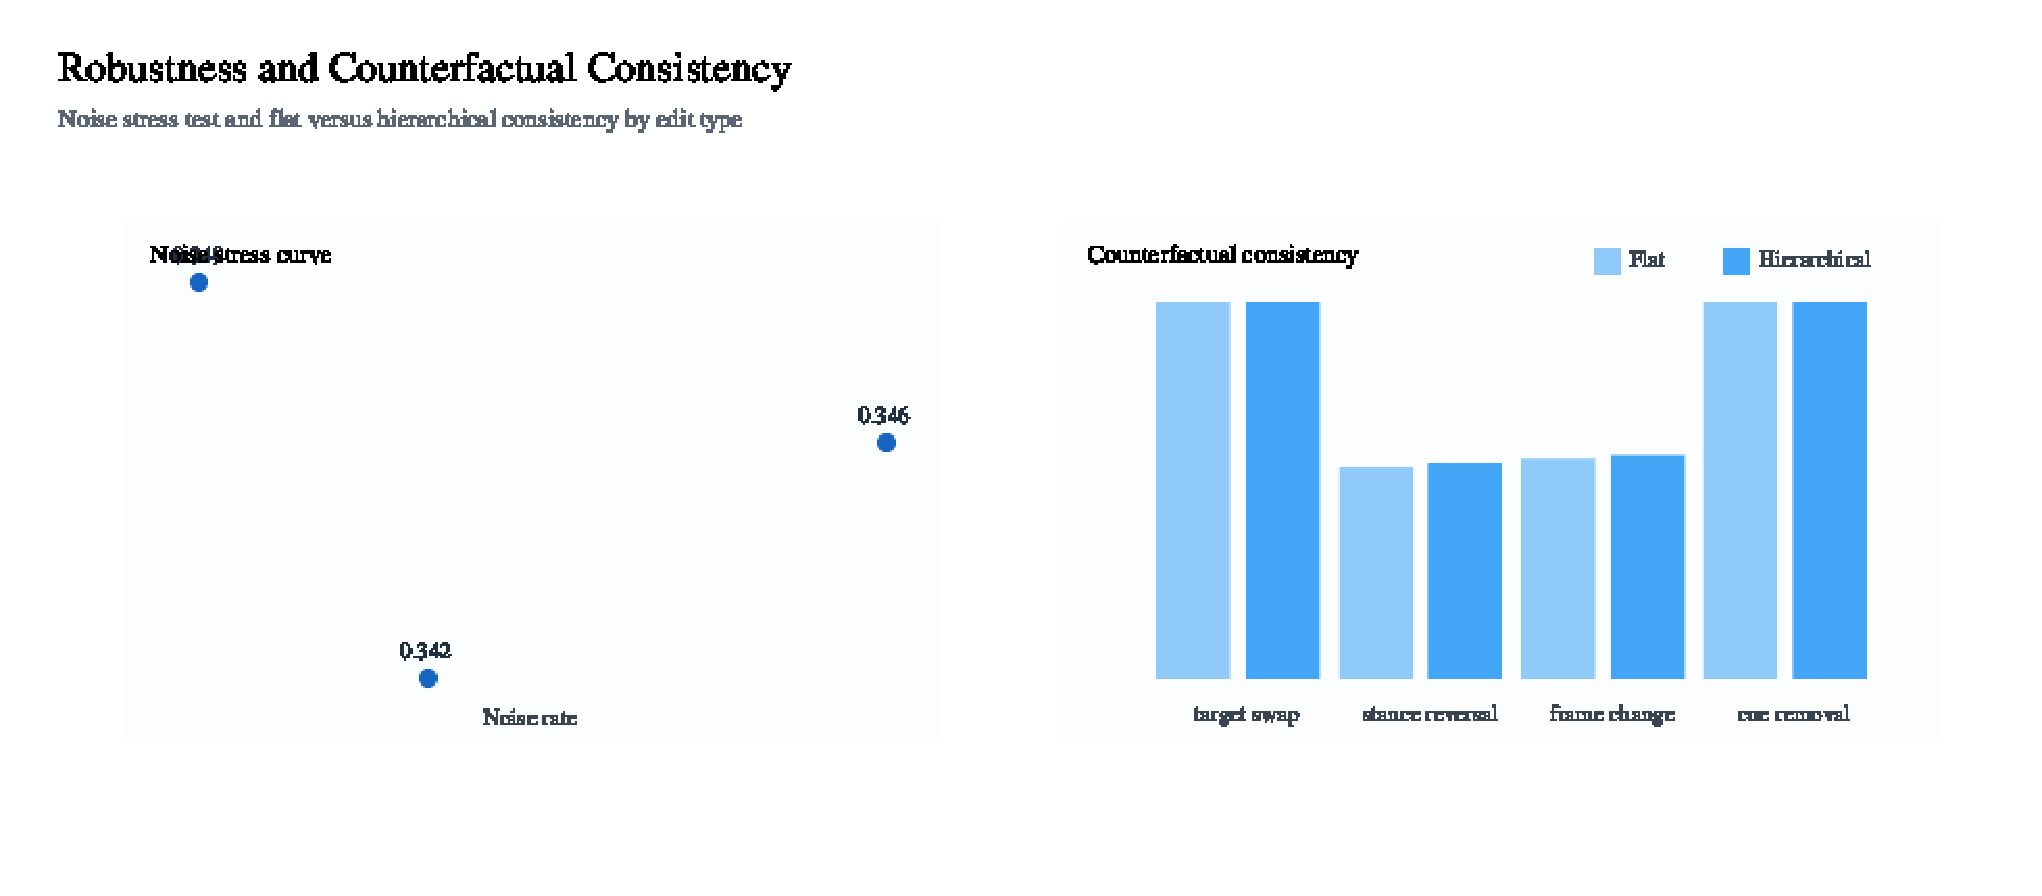
\includegraphics[width=\columnwidth]{figure03_robustness_panel.pdf}
    \caption{Robustness under noise and counterfactual edits.}
    \label{fig:robustness}
\end{figure}

The B5 and B6 comparison was verified on a small synthetic smoke setup. The smoke run used three seeds and 20 shared validation posts for the paired bootstrap comparison. It is useful for checking that prediction export, supported-label macro-F1, paired bootstrap testing, and error analysis run end-to-end. It is not a final claim about model quality. Table~\ref{tab:smoke} shows that B6 underperforms B5 under this constrained setup. Relevance is similar, but B6 is weaker on the ideology heads.

\begin{table}[t]
\centering
\small
\begin{tabular}{lcc}
\toprule
Metric & B5 & B6 \\
\midrule
Macro-F1 mean & 0.356 & 0.154 \\
Relevance & 0.467 & 0.473 \\
Economic & 0.322 & 0.194 \\
Social & 0.222 & 0.190 \\
\bottomrule
\end{tabular}
\caption{Three-seed smoke-run results for the flat and hierarchical transformer variants.}
\label{tab:smoke}
\end{table}

\begin{figure}[t]
    \centering
    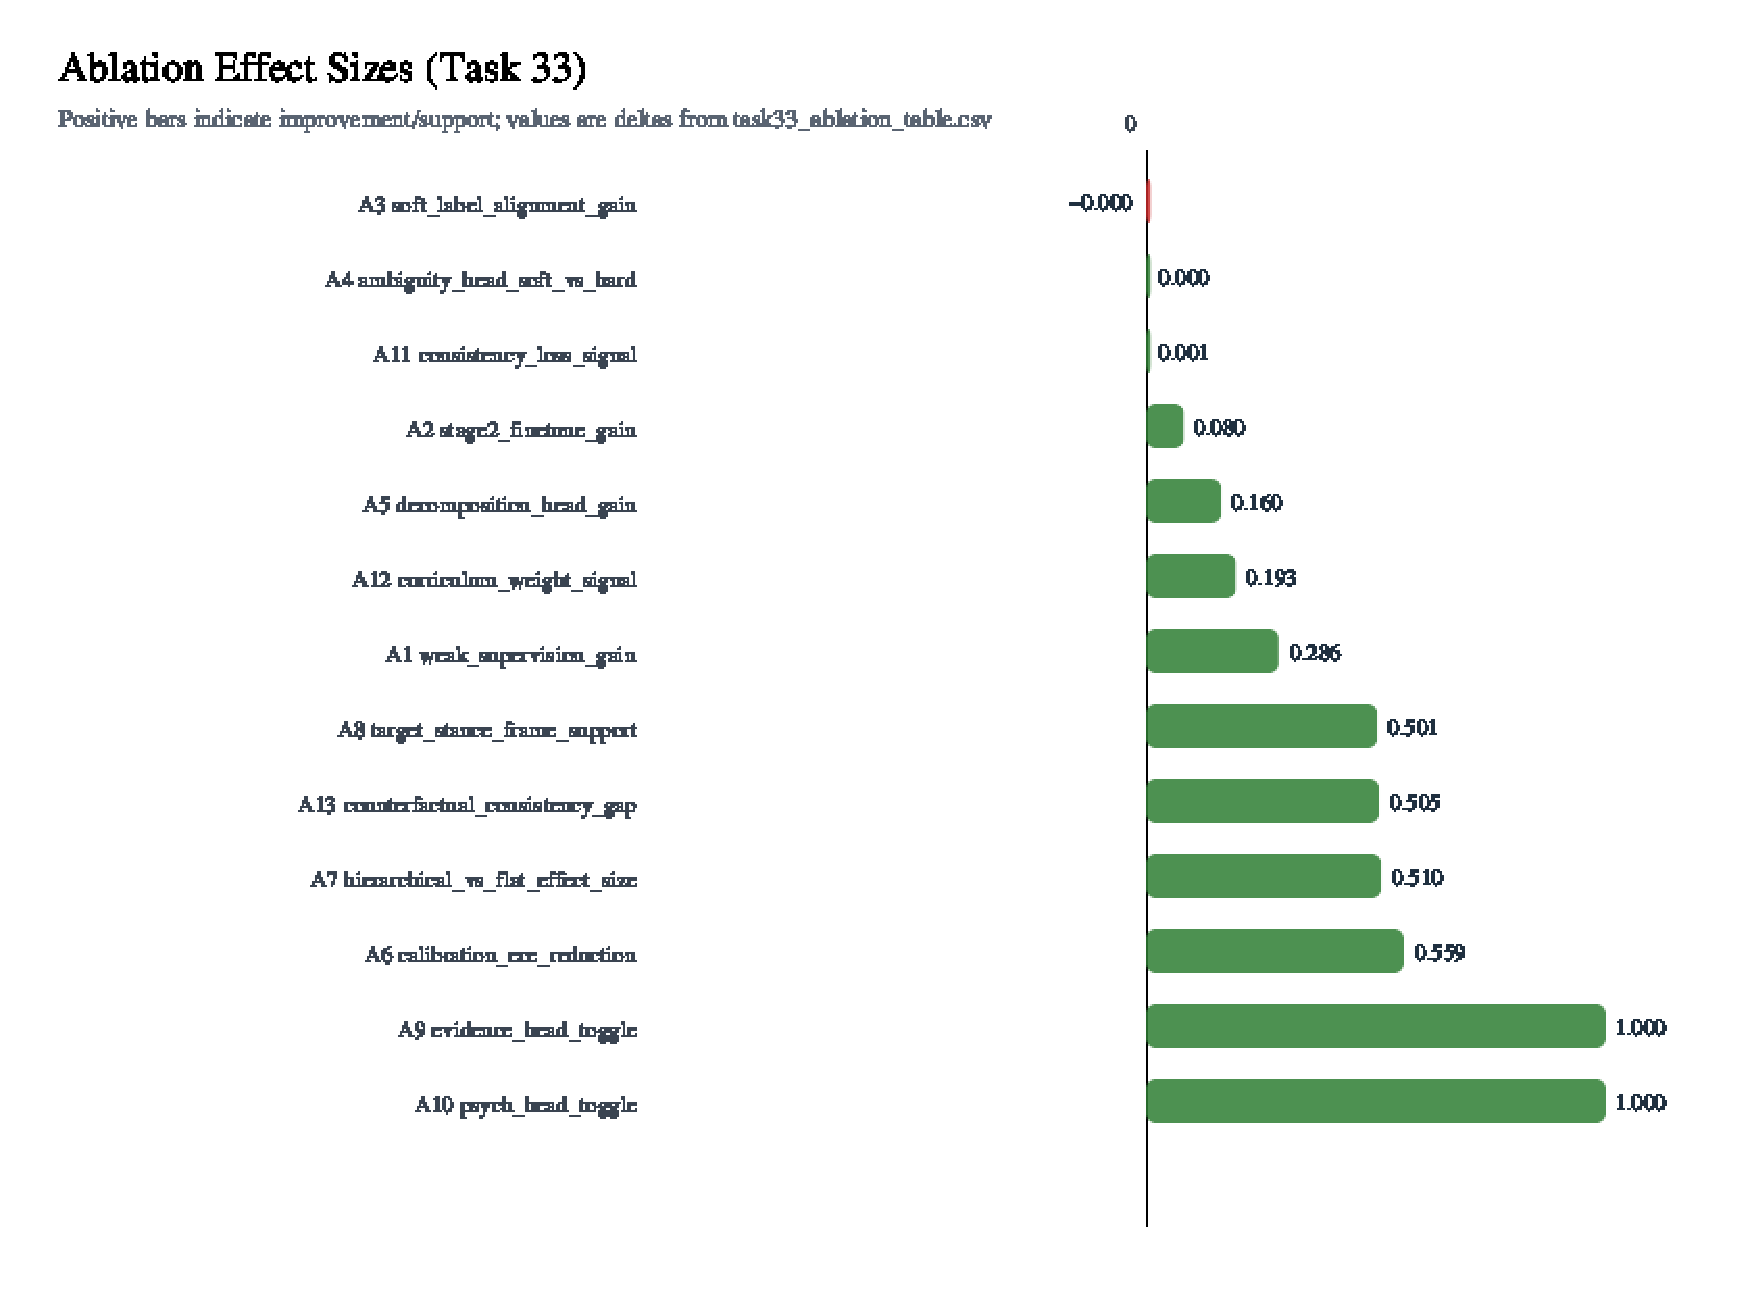
\includegraphics[width=\columnwidth]{figure02_ablation_deltas.pdf}
    \caption{Ablation deltas for model components and diagnostics.}
    \label{fig:ablation}
\end{figure}

\begin{figure}[t]
    \centering
    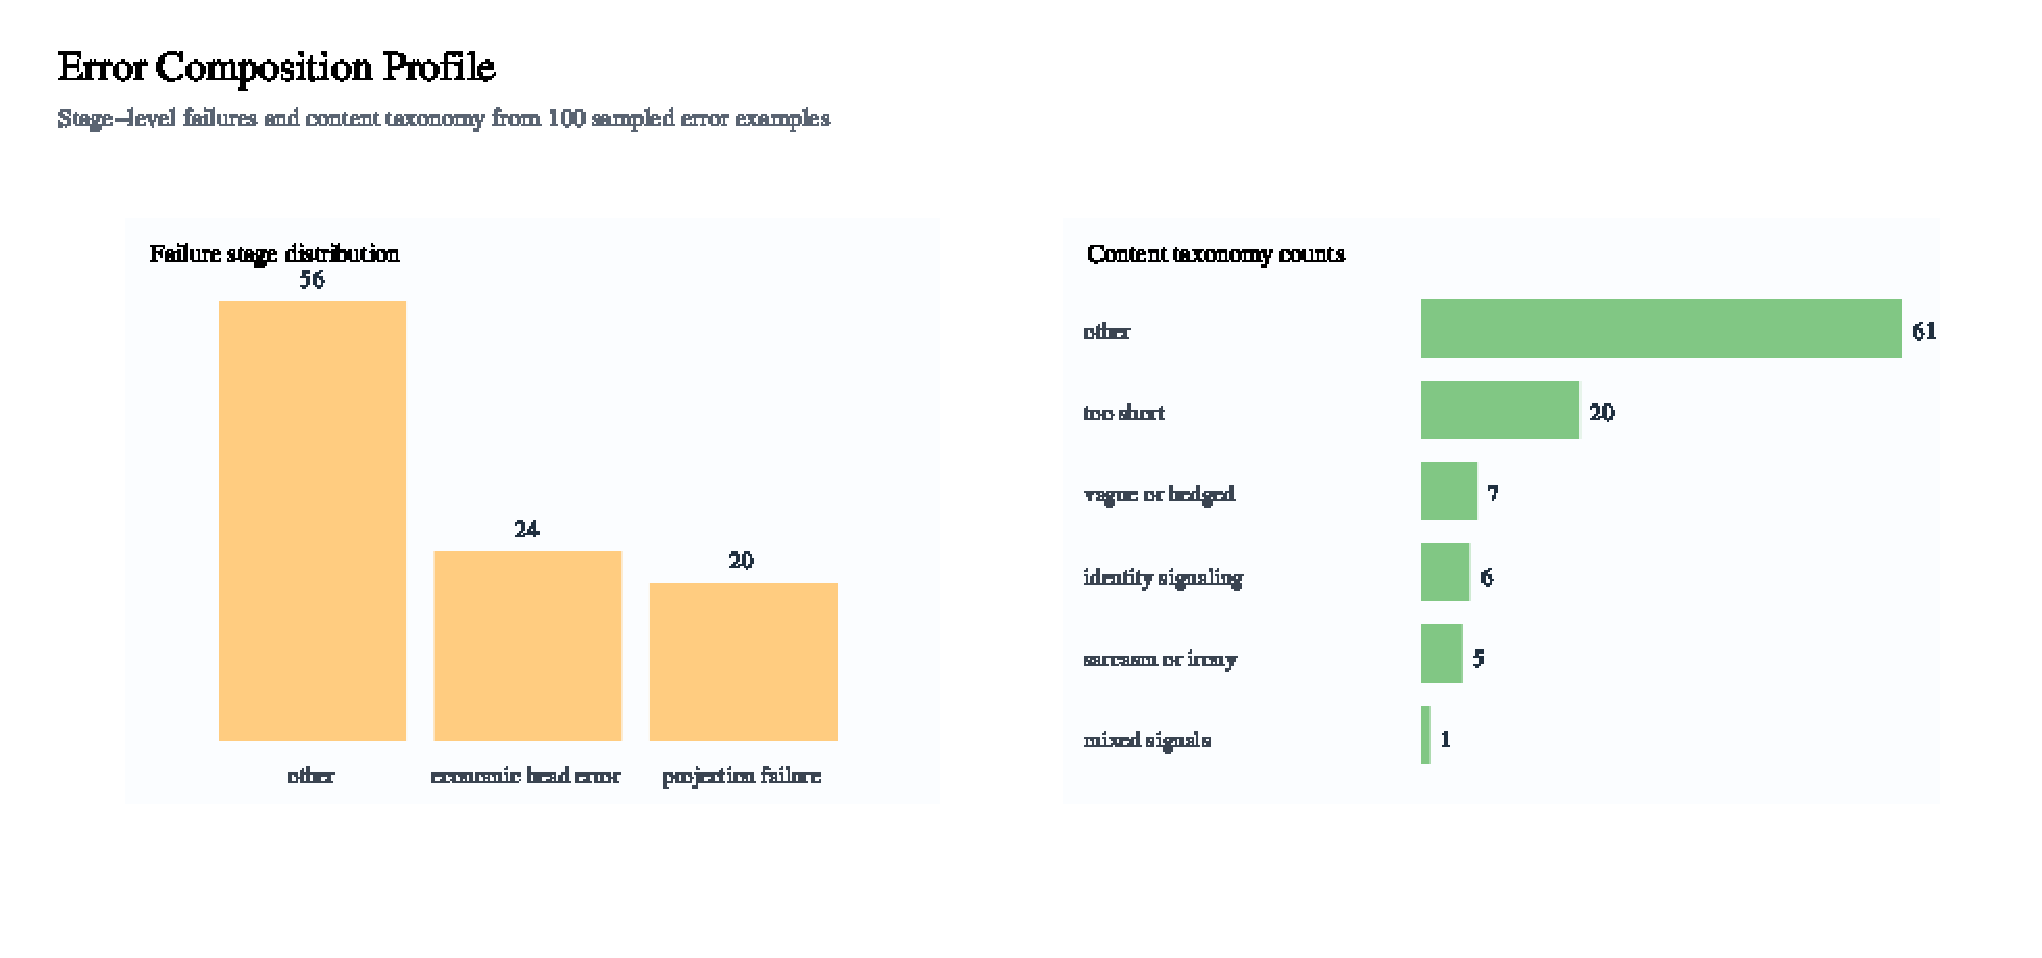
\includegraphics[width=\columnwidth]{figure04_error_profile_panel.pdf}
    \caption{Error composition by failure type and content tag.}
    \label{fig:error-profile}
\end{figure}
\FloatBarrier

\section{Limitations}

The full Reddit weak-supervision experiment could not be completed because Politosphere access was blocked in the available environment. As a result, B3 through B6 should be treated as implemented and smoke-tested rather than fully evaluated on the intended Reddit scale.

The MITweet experiment is real-data evidence, but it only covers the labels that can be cleanly projected from MITweet: relevance, economic direction, and social direction. It does not fully evaluate target, stance, frame, intensity, or ambiguity in the same way as the Reddit annotation schema.

The visualizations summarize current artifacts, but some robustness and counterfactual consistency values are diagnostics rather than direct B5 and B6 inference on every edited example. The next experimental step is class-weighted or focal loss for the ideology heads, followed by a full real-data rerun once the Reddit weak-supervision data is reachable.

\bibliographystyle{unsrtnat}
\bibliography{ideology_social_media}

\end{document}
